\documentclass[11pt]{article}
\usepackage[margin=1in]{geometry}
\usepackage{amsmath, amssymb, amsthm}
\usepackage{tikz}
\usetikzlibrary{arrows.meta, positioning}
\usepackage{booktabs}
\usepackage{microtype}
\usepackage{xcolor}
\usepackage{hyperref}
\hypersetup{colorlinks=true, linkcolor=blue!50!black, urlcolor=blue!50!black}

\newcommand{\code}[1]{\texttt{#1}}
\newcommand{\del}{\mathsf{del}}
\newcommand{\ins}{\mathsf{ins}}

\tikzset{
  vtx/.style    ={draw, circle, minimum size=7.5mm, inner sep=0pt,
                  fill=blue!8, line width=0.6pt},
  rootvtx/.style={draw, circle, minimum size=7.5mm, inner sep=0pt,
                  fill=black!12, line width=0.6pt, font=\bfseries},
  deadv/.style  ={draw, circle, minimum size=7.5mm, inner sep=0pt,
                  densely dashed, fill=black!4, text=black!40,
                  line width=0.6pt},
  anc/.style    ={-{Stealth[length=2.2mm]}, line width=0.8pt},
  elbl/.style   ={font=\scriptsize, text=black!60},
  capt/.style   ={font=\small\itshape, text=black!75},
  stbox/.style  ={draw, rounded corners=2pt, inner sep=3.5pt,
                  font=\small, fill=blue!4, line width=0.6pt},
}

\title{\bfseries Convergence Is Not Correctness\\[2pt]
\large The sequential-specification campaign: independent, kernel-checked
specs\\ for every replicated data type in Sal}
\author{Sal / FP Launchpad (KC + Claude)}
\date{2026-07-16}

\begin{document}
\maketitle
\sloppy

\begin{abstract}
\noindent
Replication-aware linearizability certifies that every version of a
replicated data type is the fold of some delivery-respecting
linearization of its events. The reference point of that guarantee is
the datatype's \emph{own} fold: a bug in \code{do} appears identically
on every replica, converges perfectly, and passes every convergence
theorem. This note records the campaign that closes the gap: for every
production RDT in Sal, a kernel-checked theorem that the fold of any
single-replica history equals the output of a straightforward
sequential program, the one a programmer would write with no
replication in mind, discovered through an explicit inductive
invariant. Four tiers, easiest to hardest: eleven flat datatypes, the
mergeable queue against a plain functional queue, the embedded-chain
RGA against the naive insert-at-index text buffer, and fused Peritext
against a naive marked-text editor. The campaign's negative results
carry as much information as its theorems: the rehoming tombstone-free
RGA is \emph{refuted} at this specification on a four-op single-replica
trace, its fused Peritext inherits the refutation at the render, and
Shesha passes sequentially while failing at the merge; together they
witness that do-faithfulness and merge-faithfulness are independent
axes. A final section states honestly what the campaign does
\emph{not} give: per-replica soundness and convergence do not compose
into ``the merged state is some user's sequential result,'' and the
precise corner where composition fails is the same dead-anchor corner
the sequence-CRDT trilemma names. Every theorem is kernel-clean; every
claim names its Lean identifier.
\end{abstract}

\section{The specification gap}
\label{sec:gap}

The framework's central guarantee is RA-linearizability at every
reachable configuration: each version the store registers is
$\mathrm{fold}(\rho)$ for some enumeration $\rho$ of the version's
event set that respects delivery order. This is a strong convergence
guarantee and it is the right one for replication: it says the merge
invented nothing, reordered nothing it was not entitled to reorder,
and that all replicas agree.

It says nothing about whether the fold is \emph{right}. The reference
sequence is the datatype's own \code{do}; if \code{do} is wrong, every
replica is wrong in unison, and RA-linearizability holds vacuously
over the shared mistake. Two incidents made this concrete in this
repository. First, a mark-extent defect in an early Peritext render
passed every convergence obligation and was caught only by eye.
Second, and decisively: the rehoming tombstone-free RGA carries a
fully general, kernel-clean RA-linearizability capstone
(\code{rga\_ra\_linearizable3\_eq}), and its \code{do} nonetheless
reorders survivors when an interior node is deleted, with no
concurrency anywhere in the history (\S\ref{sec:negative}). Both
defects are invisible to convergence because convergence is
self-referential.

The remedy is an independent specification. For sequential behaviour
there is an obvious and canonical one: \emph{the sequential program a
programmer would write for the same operations with no replication in
mind}. A counter is addition. A queue is a list. A text buffer is
insert-at-position and delete. A marked-text editor is a buffer of
characters and boundary tokens with one left-to-right walk. The
campaign's obligation, per datatype:

\begin{center}
\begin{tabular}{c}
\emph{for every sequentially honest single-replica history $\rho$:}\\[2pt]
$\mathrm{read}(\mathrm{fold}(\rho)) \;=\;
 \mathrm{specProgram}(\rho)$
\end{tabular}
\end{center}

\noindent proved by discovering an inductive invariant of the fold,
never by weakening the spec to match the implementation.
``Sequentially honest'' is the datatype's own issuing discipline
specialized to a linear history (fresh monotone stamps, each op
applicable at the state it executes against), so the theorems attack
no strawman: the histories quantified over are exactly the ones a
single well-behaved replica produces.

\section{The four tiers and their invariants}
\label{sec:tiers}

The campaign ran easiest to hardest, and the difficulty gradient
turned out to be a gradient of \emph{invariant kinds}.

\paragraph{Tier 1: the flat datatypes (eleven RDTs).}
\code{SeqSpec\_Flat.lean}. For most flat datatypes the fold is a view
homomorphism and the invariant is trivial: the counter and PN-counter
fold to arithmetic (\code{ioc\_seq\_sound},
\code{pn\_seq\_sound}), the grow-only set and map to naive
insertion (\code{goset\_seq\_sound}, \code{gomap\_seq\_sound}), the
OR-set and its efficient variant to a membership view
(\code{orset\_seq\_sound}, \code{orsete\_seq\_sound}), the
enable-wins flag and conditional G-set likewise
(\code{ewflag\_seq\_sound}, \code{gsetcond\_seq\_sound}), the LWW and
FWW registers to last- and first-write selection
(\code{lww\_seq\_sound} via the stamp-order invariant
\code{lww\_fold\_lt}, \code{fww\_seq\_sound}). Two datatypes need
genuine \emph{identity-hygiene} invariants, facts about tag bookkeeping
that hold on every reachable single-replica state and are exactly what
the induction needs: the multi-valued register's overwritten tags are
always a subset of previously staked tags (\code{mvr\_over\_tags},
feeding \code{mvr\_seq\_sound}), and the add-wins priority queue's
stake tags stay duplicate-free (\code{awpq\_mem\_seq\_sound},
\code{awpq\_inc\_log\_sound}).

\paragraph{Tier 2: the mergeable queue = a plain FIFO.}
\code{MergeableQueue\_SeqSpec.lean}: \code{queue\_seq\_sound}, with
the identity-hygiene invariant \code{q\_tags\_nodup}. Notably lean:
its axiom audit is $\{\mathrm{propext}, \mathrm{Quot.sound}\}$, with
no choice anywhere.

\paragraph{Tier 3: the embedded-chain RGA = the naive text buffer.}
\code{EmbedRGA\_SeqSpec.lean}: \code{embed\_seq\_sound}. Here the
invariant becomes \emph{geometric}. The spec program splices an insert
immediately after its anchor; the datatype sorts records by birth-chain
coordinates. The bridge is the \textbf{adjacency lemma}
(\code{chainBefore\_snoc\_iff}): a fresh insert's chain
$c_a \mathbin{+\!\!+} [\delta]$ sits directly after its anchor's chain
$c_a$ in display order, because the fresh timestamp gap $\delta$
exceeds every delta any existing chain hangs off $c_a$, a fact that
costs only sum-telescoping over the chain (every chain's deltas sum to
its id, and every existing id is below the fresh stamp). The sorted
canonical state then \emph{is} the spec buffer, record for record.
Because the published tombstoned RGA is read-equivalent to the embed
on honest event sets (the compaction theorem), it inherits the buffer
spec as a corollary: \code{rga\_seq\_read\_eq\_buffer} and the
element-level \code{rga\_seq\_read\_element}
(\code{EmbedRGA\_SeqSpec\_RGA.lean}, a standalone build target because
the two RGA models share top-level names). And because the sided
generalization simulates the one-sided instance on all-R histories
unconditionally (\code{sFold\_liftOp}), the buffer spec transports to
the sided datatype's all-R fragment at zero proof cost.

\paragraph{Tier 4: fused Peritext = a naive marked-text editor.}
\code{PeritextEmbed\_SeqSpec.lean}: \code{peritextEmbed\_seq\_sound}
and the id-tagged \code{peritextEmbed\_seq\_sound\_ids}. The editor is
a plain buffer of $(\mathrm{id}, \mathrm{element})$ entries, elements
being characters or mark boundaries, with one left-to-right walk
maintaining the open-mark set: a start boundary opens its mark, the
matching close removes it, characters display with whatever is open.
The theorem is a \emph{composition}, and that is the finding: tier 3's
buffer soundness, made payload-generic, already says the fold's
$(\mathrm{id}, \mathrm{element})$ sequence is the naive buffer, and
the datatype's render and the editor's screen are literally the same
pure fold over that sequence. No new invariant was needed. This is
also why the tier had to wait for the re-based Peritext
(\S\ref{sec:negative}): against the rehoming kernel the same statement
is false.

The gradient, summarized: \emph{identity hygiene} (tags are staked,
tags are nodup) for the flat and queue tiers, \emph{geometry}
(adjacency, stamp monotonicity) for the sequence tier,
\emph{composition} (buffer $\times$ shared render fold) for rich text.

\section{The specifications, stated}
\label{sec:specs}

This section writes out the sequential specification of every RDT in
the campaign, and flags, per datatype, where the RDT's operation
alphabet had to \emph{bend away} from the purely sequential data
structure's interface. That bend is the campaign's most instructive
artifact. A sequential structure addresses its state positionally or
implicitly: \code{dequeue()} takes no argument because ``the head'' is
unambiguous; \code{insert(i, e)} names an index. A replicated datatype
cannot, because positions and implicit referents are not stable under
concurrent edits. So the RDT operation carries a \textbf{witness}: the
identity (tag, stamp, id, coordinate, snapshot) of what the issuing
replica \emph{observed} the positional referent to be, at its own
state, at issue time. The sequential-honesty side conditions of
\S\ref{sec:tiers} are then exactly the statement ``the witness is what
the sequential operation would have seen,'' and each theorem says:
under that discipline, the witnessed-identity program implements the
positional program. Where no witness is needed, the op alphabets
coincide and the spec is a view homomorphism.

\subsection{No gap: the alphabets already coincide}

For nine of the flat datatypes the RDT op is literally the sequential
op; the state carries invisible bookkeeping (tags, per-replica slots)
and the spec is the evident program on the user-visible view.

\begin{itemize}
\item \textbf{Counter / increment-only counter.} Spec state $\mathbb{Z}$
  (resp.\ $\mathbb{N}$); $\ins\mathsf{c}$ is $n \mapsto n+1$. Theorem:
  the fold \emph{is} the history length
  (\code{counter\_seq\_sound}, \code{ioc\_seq\_sound}).
\item \textbf{PN-counter.} Spec: $\#\mathsf{inc} - \#\mathsf{dec}$
  (\code{pnSpec}); \code{pn\_seq\_sound}.
\item \textbf{Grow-only set / map, conditioned G-set.} Spec:
  accumulation; membership of $x$ iff some op added $x$
  (\code{goset\_seq\_sound}, \code{gomap\_seq\_sound},
  \code{gsetcond\_seq\_sound}).
\item \textbf{OR-set (plain and efficient).} Spec state: a plain set;
  $\mathsf{add}\,e$ inserts, $\mathsf{rem}\,e$ deletes
  (\code{orSpecStep}). The tag machinery (fresh $(t,e)$ stakes,
  filter-all-tags on remove) is invisible to one replica: the element
  view of the fold is the naive program
  (\code{orset\_seq\_sound}, \code{orsete\_seq\_sound}). No invariant
  needed; the view is a fold homomorphism.
\item \textbf{Enable-wins flag.} Spec state: one boolean;
  $\mathsf{enable} \mapsto \mathsf{true}$,
  $\mathsf{disable} \mapsto \mathsf{false}$ (\code{ewSpecStep});
  \code{ewflag\_seq\_sound}.
\item \textbf{Add-wins priority queue.} Two-part spec pinning both
  state components: membership behaves as the plain add/remove set
  with $\mathsf{inc}$ inert (\code{awpqSpecStep},
  \code{awpq\_mem\_seq\_sound}), and the increment component is a
  grow-only log of exactly the issued increments
  (\code{awpq\_inc\_log\_sound}).
\end{itemize}

\subsection{Gap: arbitration by stamp instead of program order}

\textbf{LWW and FWW registers.} The sequential register is
$\mathsf{write}\,v$ with \emph{program order} deciding who wins: the
spec programs are ``the last write's value''
(\code{lwwSpecFold}: $\_\,, o \mapsto \mathsf{some}\,(\mathrm{val}\,o)$)
and ``the first write's value'' (\code{fwwSpecFold}). The RDT op
carries its Lamport stamp \emph{as the arbitration key in the payload}
(a max- resp.\ min-semilattice on stamped writes), because concurrent
replicas have no shared program order to appeal to. The gap is the
transfer of ordering authority from control flow to data. The honesty
condition is precisely its repair: \code{stampsMono} (stamps strictly
increase along the history, the sequential Lamport condition), under
which the arbitration key agrees with program order and
\code{lww\_seq\_sound} / \code{fww\_seq\_sound} recover last-write and
first-write semantics. Without \code{stampsMono} the statements are
false and should be: a replica that back-dates a write is asking LWW
to disagree with program order.

\subsection{Gap: overwrite by snapshot instead of ``everything''}

\textbf{Multi-valued register.} The sequential register's
$\mathsf{write}\,v$ implicitly overwrites \emph{everything before it}.
The RDT op is $\mathsf{write}\,(v, O)$ where $O$ is a
\textbf{prepare-time snapshot}: the set of write-stamps the issuer
currently sees, named explicitly so that a \emph{concurrent} write
(not in $O$) survives, which is the whole point of an MVR. The
sequential spec is still the plain last-write register
(\code{mvrSpecFold}). Honesty (\code{mvrOK}): the op's stamp is fresh
and $O$ lists \emph{exactly} the issuer's visible stamps, the formal
form of ``I overwrite precisely what I can see.'' Under it,
\code{mvr\_seq\_sound}: the visible-value view of the fold is the last
write. The proof needs the campaign's first genuinely discovered
invariant, \code{mvr\_over\_tags}: every overwritten stamp was staked,
which is what makes a fresh stamp provably not-yet-overwritten.

\subsection{Gap: dequeue() becomes delete-what-I-saw}

\textbf{The mergeable queue}, the cleanest specimen of the principle.
The sequential queue is
\[
  \mathsf{enq}\,v : S \mapsto S \mathbin{+\!\!+} [v]
  \qquad\qquad
  \mathsf{deq}() : S \mapsto \mathrm{tail}(S)
\]
with \code{deq} \emph{nullary}: the head is implicit. The RDT cannot
say ``the head'' (two replicas may disagree about it), so its op is
$\mathsf{deq}\,t$: remove \emph{by tag}, where $t$ is the tag of the
element the issuing replica read as the head of \emph{its own} queue.
The implementation filters $t$ out of the whole list, wherever it
sits. The spec keeps the sequential shape, \code{tail}, blind to $t$
(\code{qSpecStep}); honesty (\code{qOK}) says the witness is faithful:
the fold at the issue point is literally $(t, v) :: \mathit{rest}$.
The invariant \code{q\_tags\_nodup} (fresh stakes stay
duplicate-free) makes filter-by-tag remove exactly the head, and
\code{queue\_seq\_sound} closes the loop: delete-what-I-saw implements
pop-the-head. The same witness discipline is what the convergence side
already consumed (\code{qHonest\_of\_applicable}); the campaign reuses
the datatype's own contract rather than inventing one.

\subsection{Gap: insert-at-index becomes insert-after-who-I-saw}

\textbf{The embedded-chain RGA.} The sequential text buffer is
$\mathsf{insert}(i, e)$ and $\mathsf{delete}(i)$, index-addressed. The
RDT op is $\ins(e, \pi, a)$: $a$ is the \emph{id} of the element the
issuer saw at position $i - 1$ (the anchor; the sentinel $0$ for the
head), and $\pi$ is the anchor's stored coordinate as the issuer read
it (the proof-carrying prefix); $\del(x)$ names the id seen at
position $i$. The spec program is the buffer in id-clothing
(\code{eSpecStep}): front-cons for $a = 0$, otherwise splice
immediately after $a$'s entry (\code{eInsAfter}); delete filters by
id. On a sequential history the anchor id determines the index
uniquely, so this \emph{is} the positional program with positions
named by their occupants. Honesty (\code{eSeqOK}): stamps exceed all
prior insert stamps, and each op is \code{eApplicable} at the current
fold, i.e.\ the anchor is live and carries exactly $\pi$: the witness
is faithful. The theorem (\code{embed\_seq\_sound}) is the strongest
form in the campaign: the canonical sorted state equals the spec
buffer \emph{record for record}, via the adjacency lemma. The same
spec, verbatim, is what the rehoming RGA is refuted against
(\S\ref{sec:negative}): the gap analysis there is not about the
witness (the rehoming op carries one too, plus a path) but about the
implementation moving other elements' referents after a delete.

\subsection{Gap: one mark becomes a boundary pair}

\textbf{Fused Peritext.} The sequential marked-text editor has an
\emph{atomic} $\mathsf{mark}(i, j, m)$. The fused RDT has no such op:
a mark is \textbf{two} ordinary inserts of boundary elements
$\langle m\rangle$, $\langle/m\rangle$ sharing a fresh mark id,
anchored at the range ends, and mark removal is two deletes. The
atomic sequential op is traded for a pair of witnessed inserts, which
is the atomicity horn of the mark-positioning trilemma, accepted
knowingly. The spec therefore lives at the token level: the editor is
the tier-3 buffer over
$\mathrm{char} \oplus \mathrm{boundary}$ entries plus one
left-to-right walk maintaining the open-mark set (a start boundary
opens, the matching close removes, characters display with what is
open). \code{peritextEmbed\_seq\_sound} says the datatype's render is
that editor's screen; the range-level reading is recovered by the
positional intent theorems (\code{render\_id\_active\_iff\_between}:
a character carries mark $m$ iff it sits, in reading order, strictly
between $m$'s boundaries). The boundary-pair encoding is also why the
character/boundary distinction is load-bearing in the delete theorem:
deleting a \emph{character} re-formats nothing
(\code{renderIds\_del}), deleting a \emph{boundary} is mark removal
and must re-format its span.

\medskip
\noindent The pattern, in one sentence: \emph{every honesty condition
in the campaign is the faithfulness of a witness that replaced a
positional argument}, and the campaign's theorems are the statement
that witnessed operations, honestly issued, are positional operations.

\section{The negative rows, and the two-axis separation}
\label{sec:negative}

The campaign's statement shape is falsifiable per datatype, and three
refutations landed. All three are machine-checked.

\paragraph{The rehoming RGA fails at \code{do}.}
\code{RGA\_Rehoming/RGA\_SeqSpec\_Refuted.lean}:
\code{rehoming\_seq\_refuted}. The witness
(Figure~\ref{fig:witness}) is four ops on one replica, honest in the
datatype's own terms (every op \code{accurate} and \code{fresh\_ts} at
its state): build $\langle b, a, c\rangle$ with $c$ under $a$, then
delete $a$. The naive buffer keeps survivor order, $\langle b,
c\rangle$; the rehoming \code{do} re-homes $c$ to the root, where the
newest-first sibling tiebreak leapfrogs it over $b$: the read is
$\langle c, b\rangle$. The should-pass half
(\code{seq\_agrees\_before\_delete}) shows both sides agree on the
delete-free prefix, isolating the delete as the exact point of
departure. The design's convergence capstone is untouched: it
converges, to its own reordering fold.

\begin{figure}[h]
\centering
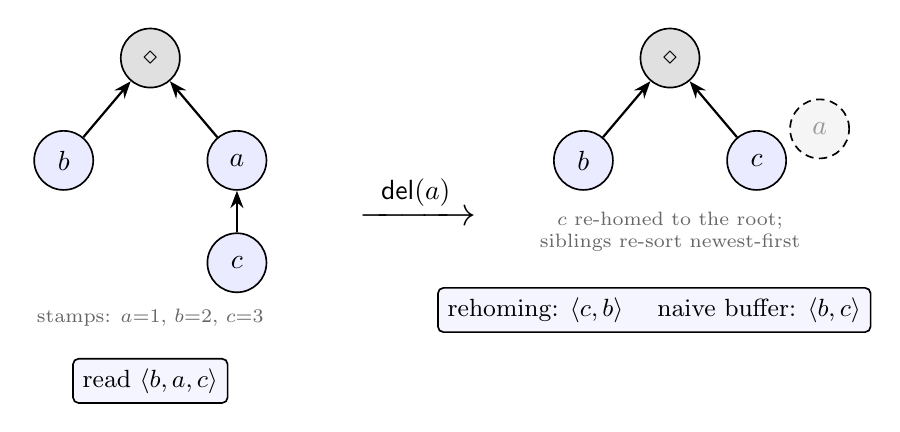
\begin{tikzpicture}
  \node[rootvtx] (r) at (0,0) {$\diamond$};
  \node[vtx] (b) at (-1.1,-1.3) {$b$};
  \node[vtx] (a) at (1.1,-1.3) {$a$};
  \node[vtx] (c) at (1.1,-2.6) {$c$};
  \draw[anc] (b) -- (r);
  \draw[anc] (a) -- (r);
  \draw[anc] (c) -- (a);
  \node[elbl] at (0,-3.3) {stamps: $a{=}1$, $b{=}2$, $c{=}3$};
  \node[stbox] at (0,-4.1) {read $\langle b, a, c\rangle$};
  \node at (3.4,-1.8) {\Large $\xrightarrow{\ \del(a)\ }$};
  \begin{scope}[shift={(6.6,0)}]
  \node[rootvtx] (r2) at (0,0) {$\diamond$};
  \node[vtx] (b2) at (-1.1,-1.3) {$b$};
  \node[deadv] (a2) at (1.9,-0.9) {$a$};
  \node[vtx] (c2) at (1.1,-1.3) {$c$};
  \draw[anc] (b2) -- (r2);
  \draw[anc] (c2) -- (r2);
  \node[elbl, align=center] at (0,-2.2)
    {$c$ re-homed to the root;\\ siblings re-sort newest-first};
  \node[stbox] at (-0.2,-3.2) {rehoming: $\langle c, b\rangle$
    \quad naive buffer: $\langle b, c\rangle$};
  \end{scope}
\end{tikzpicture}
\caption{The four-op refutation trace. One replica, no merge. Deleting
$a$ swaps the surviving $b$ and $c$ in the rehoming RGA's read; the
naive text buffer keeps their order. Machine-checked as
\code{rehoming\_seq\_refuted}; the embedded-chain RGA reads
$\langle b, c\rangle$ on the same trace, because $c$'s immutable
coordinate still carries $a$'s chain as pure geometry.}
\label{fig:witness}
\end{figure}

\paragraph{Fused Peritext on the rehoming kernel fails at the render.}
\code{Peritext\_Rehoming/Peritext\_Read.lean}:
\code{fused\_delete\_reformats\_survivor}. The same reorder, lifted to
$\mathrm{char} \oplus \mathrm{boundary}$: deleting a plain character
re-homes a survivor past a mark boundary, and an untouched character
changes formatting, single-replica. This is what converted the
rehoming design's demotion from taste into obligation, and what made
the re-base of Peritext onto the embed kernel a correctness fix. On
the embed kernel the corresponding \emph{general} theorem holds:
\code{renderIds\_del} (axioms $\{\mathrm{propext},
\mathrm{Quot.sound}\}$): deleting a character leaves every other
character's rendered formatting bitwise untouched, because character
entries are open-set-neutral and delete is a filter on an
order-canonical state. Its boundary hypothesis is necessary and
machine-checked so
(\code{boundary\_delete\_breaks\_filter\_eq}): deleting a
\emph{boundary} is mark removal and rightly re-formats the span.

\paragraph{Shesha passes sequentially and fails at the merge.}
The mirror image. Shesha's single-replica reads are the naive linked
list (\code{sequential\_soundness}, kernel-clean), and it uniquely
preserves survivor order under delete among the tombstone-free designs
of its generation (\code{delete\_preserves\_survivor\_order}). Its
\emph{merge} is machine-checked non-RA-linearizable
(\code{Shesha\_Rows\_Refuted}): at an honest reachable configuration
the three-way merge splits a deleted node's children around a
concurrent sibling, producing a read that is the fold of no
delivery-respecting linearization.

\begin{figure}[h]
\centering
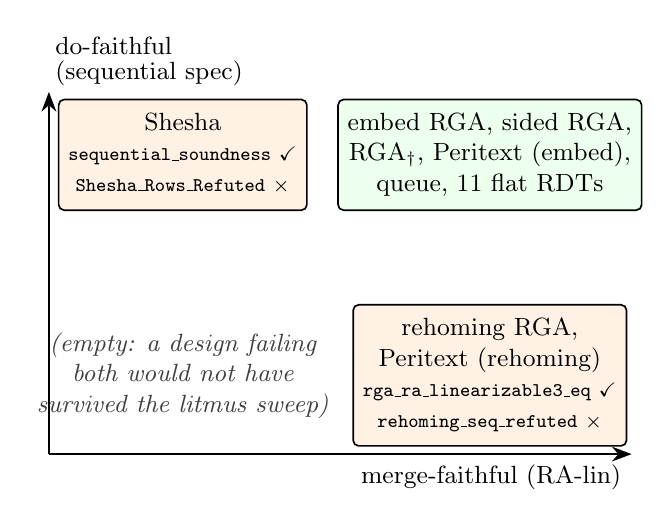
\begin{tikzpicture}[scale=1.0]
  \draw[-{Stealth[length=2.5mm]}, line width=0.9pt] (0,0) -- (7.4,0)
    node[below left, font=\small] {merge-faithful (RA-lin)};
  \draw[-{Stealth[length=2.5mm]}, line width=0.9pt] (0,0) -- (0,4.6)
    node[above right=-2pt, font=\small, align=left] {do-faithful\\[-2pt]
      (sequential spec)};
  \node[stbox, fill=green!7] at (5.6,3.8)
    {\begin{tabular}{@{}c@{}}embed RGA, sided RGA,\\
      RGA$_\dagger$, Peritext (embed),\\ queue, 11 flat RDTs\end{tabular}};
  \node[stbox, fill=orange!10] at (1.7,3.8)
    {\begin{tabular}{@{}c@{}}Shesha\\
      \scriptsize\code{sequential\_soundness} $\checkmark$\\
      \scriptsize\code{Shesha\_Rows\_Refuted} $\times$\end{tabular}};
  \node[stbox, fill=orange!10] at (5.6,1.0)
    {\begin{tabular}{@{}c@{}}rehoming RGA,\\ Peritext (rehoming)\\
      \scriptsize\code{rga\_ra\_linearizable3\_eq} $\checkmark$\\
      \scriptsize\code{rehoming\_seq\_refuted} $\times$\end{tabular}};
  \node[capt, align=center] at (1.7,1.0)
    {(empty: a design failing\\ both would not have\\ survived the
      litmus sweep)};
\end{tikzpicture}
\caption{The two-axis separation, every placement kernel-checked.
Do-faithfulness (the fold matches the naive sequential program) and
merge-faithfulness (RA-linearizability) fail independently: the
rehoming family converges to a reordering fold; Shesha folds correctly
and merges outside every linearization. The campaign's informative
content is that the top-right corner is achievable, and by the same
design idea in both sequence datatypes: immutable birth coordinates.}
\label{fig:axes}
\end{figure}

\section{What composition does not give}
\label{sec:caveat}

It is tempting to compose the two guarantees: RA-linearizability says
every version is $\mathrm{fold}(\rho)$ for some delivery-respecting
$\rho$ over the event union; the campaign says folds of sequentially
honest histories equal the spec program. May one conclude that every
merged document is the naive program's output on \emph{some} ordering
of everyone's operations? \textbf{No}, and the failure is precise.

The campaign's theorems quantify over \emph{sequentially honest}
histories: stamps monotone over inserts, every op applicable at the
fold of its own prefix. An RA-linearizability witness $\rho$ is
delivery-respecting but need not be sequentially honest on either
count. Stamp monotonicity fails harmlessly (any enumeration can be
re-sorted when the state is a function of the event set, which is
exactly fold-canonicity). Applicability is the real corner: in the
union of two branches, an insert's anchor may be deleted by a
\emph{concurrent} op carrying a smaller Lamport stamp, so in
stamp-sorted order the delete precedes the insert and the insert is
not applicable at its prefix: the naive buffer no-ops it, while the
datatype (whose coordinates travel in the op) places it correctly.
Concretely: $\ins(2 \text{ after } 1)$ concurrent with $\del(1)$.
The order $[\ins 1, \ins 2, \del 1]$ replays to $\langle 2\rangle$ on
both sides; the order $[\ins 1, \del 1, \ins 2]$ makes the buffer
drop $2$ while the fold keeps it. Some interleavings of the union
match the spec program and some do not, and \emph{whether a matching
sequentially honest interleaving always exists on honest
configurations is open}. We record it as such:

\begin{quote}
\textbf{Open question (oq:seqwitness).} On every honestly reachable
configuration of the embedded-chain RGA, does the event union admit a
delivery-respecting enumeration that is also sequentially honest (so
that the merged read is the naive buffer's output on it)? Caution from
adjacent territory: for the rehoming design, the analogous
``order dependency edges first'' discipline is refuted
(\code{DepComp}, via rehoming non-transitivity). The embed's
immutable coordinates remove the refutation's mechanism, but no proof
exists in either direction.
\end{quote}

Independently of that question, the composition that \emph{is} sound
and kernel-checked today: every version is the datatype's fold of a
delivery-respecting enumeration (RA-lin), the fold is canonical per
event set (\code{e\_fold\_canon}), each replica's own contribution
obeyed the sequential spec while it was being made (this campaign),
and merge-level intent is delivered by separate, named theorems where
it holds: delete-order preservation as sublist stability, subtree
convexity as non-interleaving, read-equivalence to the published RGA
as the compaction theorem. The campaign does not manufacture a
merge-level user story; it pins the single-replica story so that
merge-level claims have something sound to stand on.

\section{The verified matrix, consolidated}
\label{sec:matrix}

The anomaly-comparison matrix (task \#64,
\code{whiteboard/anomaly-matrix/}) ran six implementations and four
production libraries through 25{,}917 merges per row, every cell
backed by executed code. Its in-repo rows have since been upgraded
from ``machine-run'' to ``kernel-checked'': the table below is the
matrix's load-bearing core with each cell a Lean theorem. External
libraries (Yjs, Automerge, Loro, list-positions) remain empirical by
nature; their rows live in the matrix report unchanged.

\begin{center}\scriptsize
\begin{tabular}{@{}lll@{}}
\toprule
design & sequential spec (do) & RA-lin (merge) \\
\midrule
embedded-chain RGA & \code{embed\_seq\_sound} &
  \code{embed\_ra\_linearizable3} \\
sided RGA (all-R) & via \code{sFold\_liftOp} &
  \code{sided\_embed\_ra\_linearizable3} \\
published RGA$_\dagger$ & \code{rga\_seq\_read\_eq\_buffer} &
  \code{rgaWithTombstones\_ra\_lin...\_eq} \\
Peritext (embed) & \code{peritextEmbed\_seq\_sound} &
  \code{peritextEmbed\_ra\_linearizable3} \\
mergeable queue & \code{queue\_seq\_sound} &
  \code{queue\_ra\_linearizable3} \\
eleven flat RDTs & \code{*\_seq\_sound} &
  \code{*\_ra\_linearizable3\_eq} \\
\midrule
rehoming RGA & \textbf{refuted}: \code{rehoming\_seq\_refuted} &
  \code{rga\_ra\_linearizable3\_eq} \\
Peritext (rehoming) & \textbf{refuted} (render):
  \code{fused\_delete\_reformats\_surv...} &
  \code{peritext\_ra\_lin..\_eq} \\
Shesha & \code{sequential\_soundness} &
  \textbf{refuted}: \code{Shesha\_Rows\_Refuted} \\
\bottomrule
\end{tabular}
\end{center}

\noindent Axiom audits: every positive theorem above is kernel-clean
(axioms $\subseteq \{\mathrm{propext}, \mathrm{Classical.choice},
\mathrm{Quot.sound}\}$; the queue's and \code{renderIds\_del}'s audits
omit choice). Refutations by concrete witness use the SPOT convention
(\code{native\_decide}, adding the compiler axioms); the refuted
\emph{statements} are quantified properties, so each refutation
discharges its honesty guards on the witness and is not an artifact of
a malformed trace.

\section{Method notes}
\label{sec:method}

Three practices earned their keep and are recorded as convention.
\emph{Falsifiable statement first}: each tier states the equality
before any proof work, and a refutation is a first-class outcome
(three landed). \emph{The spec is external}: the sequential program is
written from the datatype's user-facing intent, never read off the
implementation; where the two disagree, the disagreement is the
result. \emph{PASS and FAIL shaped tests}: every concrete SPOT block
carries should-fail companions with hand-derived expected values (the
wrong answer asserted wrong), so the harness demonstrably
discriminates; the campaign's own refutation files pair each negative
with the positive prefix on which the sides still agree, isolating the
departing operation exactly.

\paragraph{Mechanization map.} Tier 1:
\code{MRDT\_Instances/SeqSpec\_Flat.lean}. Tier 2:
\code{MergeableQueue/MergeableQueue\_SeqSpec.lean}. Tier 3:
\code{EmbedRGA/EmbedRGA\_SeqSpec.lean} and
\code{EmbedRGA/EmbedRGA\_SeqSpec\_RGA.lean} (standalone target).
Tier 4: \code{Peritext\_Embed/PeritextEmbed\_SeqSpec.lean}. Negative
rows: \code{RGA\_Rehoming/RGA\_SeqSpec\_Refuted.lean},
\code{Peritext\_Rehoming/Peritext\_Read.lean} \S10,
\code{Shesha/Shesha\_Rows\_Refuted.lean}. The render fix theorem:
\code{Peritext\_Embed/PeritextEmbed.lean}. All paths relative to
\code{Sal/ConditionedMRDTs/}.

\end{document}
